\documentclass[../../main/main.tex]{subfiles}
\begin{document}
\section{Introduction}

Poker is a notoriously complex game, with many different variants and strategic elements that have challenged both players and theorists for decades. Simplified poker models play a crucial role in game theory research by isolating specific strategic aspects---such as bluffing, value betting, and bet sizing---while remaining analytically tractable. One such class of models is Continuous Poker, which abstracts poker hands to continuous numerical hand strengths and restricts play to a single betting round. This simplification allows for exact Nash equilibrium solutions and provides insights that can inform understanding of more complex poker variants.

In this paper, we introduce and analyze Limit Continuous Poker (LCP), a new variant that bridges two well-studied extremes: Fixed-Bet Continuous Poker (FBCP), where the bettor must choose a predetermined bet size, and No-Limit Continuous Poker (NLCP), where the bettor can choose any positive bet size. LCP generalizes both by imposing lower and upper bounds $L$ and $U$ on allowable bet sizes, creating a spectrum of games parametrized by these limits.

\subsection{Related Work and Background}

The study of simplified poker models dates back to von Neumann's seminal work on game theory, which introduced the concept of optimal mixed strategies in competitive games. Continuous poker variants have since become standard examples in game theory textbooks and research, serving as tractable models for studying information asymmetry and strategic bluffing. Our work builds directly on two classical variants: Fixed-Bet Continuous Poker (FBCP) and No-Limit Continuous Poker (NLCP). We briefly review these games to establish context for LCP.

\subsubsection{Fixed-Bet Continuous Poker (FBCP)}

Continuous Poker (also called Von Neumann Poker, and referred to in this paper as Fixed-Bet Continuous Poker or FBCP) is a simplified model of poker introduced by von Neumann. It is a two-player zero-sum game designed to study strategic decision-making in competitive environments. The game abstracts away many complexities of real poker, focusing instead on the mathematical and strategic aspects of bluffing, betting, and optimal play.

\begin{definition}[FBCP]
Two players, referred to as the bettor and the caller, each put a 0.5 unit ante into a pot\footnote{An ante of 1 is often used, but since the pot size is the more relevant value, we use an ante of 0.5. All bet sizes scale proportionally.}. They are each dealt a hand strength between 0 an 1 (referred to as $x$ for bettor and $y$ for caller). After seeing $x$, the bettor can either check - in which case, the higher hand between $x$ and $y$ wins the pot of 1 and the game ends - or they can bet, by putting a pre-determined amount $B$ into the pot. The caller must now either call by matching the bet of $B$ units, after which the higher hand wins the pot of $1+2B$ minus their ante of $0.5$, or fold, conceding the pot of $1+B$ to the bettor and ending the game.
\end{definition}

FBCP has many Nash equilibria, but it has a unique one in which the caller plays an admissible strategy\footnote{An admissible strategy is one which is not weakly dominated by any other strategy.}, as shown by Ferguson and Ferguson \cite[p. 2]{ferguson2003borel}. This strategy profile, parametrized by the bet size $B$, is as follows:

The bettor bets with hands $x$ such that either 

$$x > \frac{1 + 4B + 2B^2}{(1+2B)(2+B)} \text{ or } x < \frac{B}{(1+2B)(2+B)}. $$

We call the higher interval the value betting range and the lower interval the bluffing range. The caller calls with hands $y$ above a calling threshold:

$$ y > \frac{B(3 +2B)}{(1+2B)(2+B)}. $$

Note that uniqueness in this context ignores the strictness of inequalities, since the endpoints of intervals occur with probability 0. The non-uniqueness of this Nash Equilibrium is due to the fact that given the bettor's strategy, the caller has many optimal responses. The caller must always fold with hands below the bluffing threshold, and must always call with hands above the value betting threshold, but with hands inbetween, they are indifferent between calling and folding. This is because with a hand strength in this range, the caller wins if and only if the bettor is bluffing, so their actual hand strength is irrelevant as long as it beats the bluffing threshold. To prevent the betting player from exploiting them, the caller need only call with exactly the right proportion of hands in this range. For example, the caller could take the strategy described above, but swap some calling and folding hands in the range between the bluffing and value betting thresholds.

Why is this Nash equilibrium special? We mentioned above that it is admissible, meaning that both players' strategies are not weakly dominated by any other strategy. Importantly, the caller's strategy is not weakly dominated. The same cannot be said for other Nash equilibria like the one described in the previous paragraph, for reasons that are beyond the scope of this introduction but relate to themes in Section \ref{subsec:monotone_strategies}.

FBCP also has a unique value as a function of the bet size $B$. The value of the game for the bettor is 

$$ V_{FB}(B) = \frac{B}{2(1+2B)(2+B)}, $$

which is positive (advantageous to the bettor) and maximized at $B = 1$, when the bet size is exactly the pot size. It should not be surprising that the value is positive - at worst, the bettor can always check and turn the game into a coin flip, so the bettor will only deviate from this strategy if they have a positive expected value. The fact that $B=1$ exactly maximizes the value is more subtle, but we should expect that some such maximal value of $B$ exists. Forcing the bettor to bet too large relative to the pot would make betting too risky with most hands, and making the bet too small would simply give less profit to the bettor when they win a bet. As we will see later, part of the motivation for studying LCP is to understand this concept more generally.

\subsubsection{No-Limit Continuous Poker (NLCP)}
Another continuous poker variant allows the bettor to choose a bet size $s > 0$ after seeing their hand strength, as opposed to a fixed bet size $B$. This variant is called No-Limit Continuous Poker (or Newman Poker after Donald J. Newman, or NLCP in this paper). The Nash equilibrium strategy profile for this variant is discussed and solved by Bill Chen and Jerrod Ankenman \cite[p. 154]{chen2006mathematics}.

In Nash Equilibrium, the bettor should make large bets with their strongest and weakest hands and smaller bets or checks with their intermediate hands. It turns out that the optimal strategy is most elegantly described by a mapping from bet sizes $s$ to hand strengths $x$ for bluffing and value betting, respectively\footnote{This feels backwards - mapping hand strengths to bet sizes would be more natural, but the math is more elegant this way.}. The caller simply has a calling threshold $c(s)$ for each possible bet size $s$. The full strategy profile is as follows:

The bettor bets $s$ with hands $x$ such that either

$$ x = \frac{3 s+1}{7 (s+1)^3} \text{ or } x = 1 - \frac{3}{7 (s+1)^2}, $$

where the first condition represents bluffing hands and the second value betting hands. After seeing a bet of size $s$, the caller should call with hands $y$ such that

$$ y > 1 - \frac{6}{7 (s+1)}. $$

See Figure \ref{fig:nlcp_strategy_profile} for a graphical representation of the strategy profile.

\begin{figure}[h!]
    \centering
    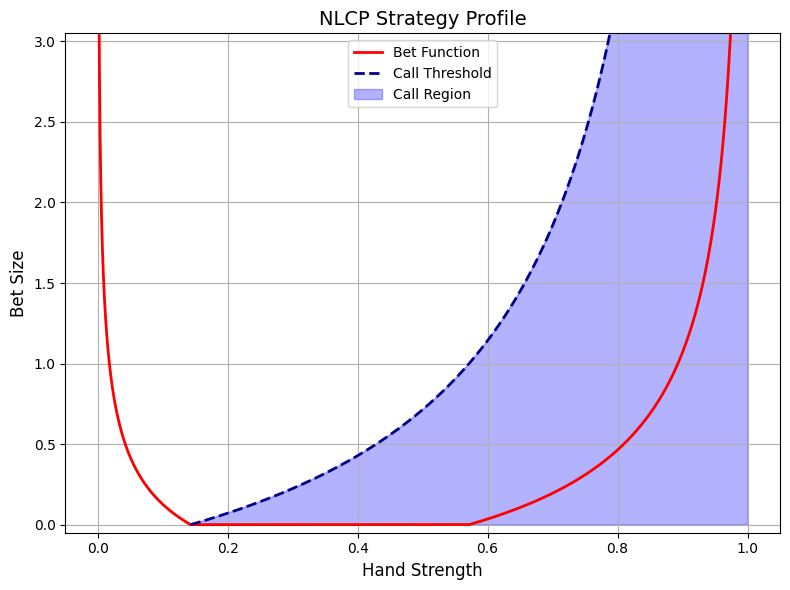
\includegraphics[width=0.8\textwidth]{images/NLCP_strategy_profile.png}
    \caption{NLCP Strategy Profile}
    \label{fig:nlcp_strategy_profile}
\end{figure}

Note that the bettor uses all possible bet sizes and has exactly two hand strengths for each bet size\footnote{Seen visually in Figure \ref{fig:nlcp_strategy_profile} by the fact that a horizontal line intersects the bet function at exactly two points.}. On first inspection, this feels like the bettor is giving away too much information, but it turns out to still be an optimal strategy. This concept appears again and is explained more thoroughly in Section \ref{subsec:nash_equilibrium_structure}.

The value of NLCP is

$$ V_{NL} = \frac{1}{14}, $$

for the bettor\footnote{Would be 1/7 for an ante of 1, but the value is halved with an ante of 0.5.}. Thus, NLCP is again advantageous to the bettor. In fact, one can easily verify that NLCP is more advantageous to the bettor than FBCP for any bet size $B$ by arguing that the bettor could artificially restrict themselves to a single bet size and achieve the same value as the bettor in FBCP.

Ferguson and Ferguson \cite{ferguson2003borel} provided the comprehensive analysis of FBCP described above, establishing the unique admissible Nash equilibrium and deriving closed-form solutions for optimal strategies. Chen and Ankenman \cite{chen2006mathematics} extended this analysis to NLCP, demonstrating how unlimited bet sizing fundamentally changes the strategic landscape while maintaining analytical tractability. Our work builds on these foundations by introducing a parametric family of games that interpolates between these extremes, allowing us to study how betting constraints affect optimal strategies and game value in a continuous fashion.

\subsection{Our Contributions}

This paper makes the following contributions:

\begin{itemize}
    \item \textbf{Nash Equilibrium Solution:} We derive the unique admissible Nash equilibrium for LCP, characterized by six threshold parameters and two continuous bet-sizing functions. We establish the structure of optimal play and provide closed-form expressions for all strategic components (Section \ref{subsec:nash_equilibrium_structure} and Section 3).

    \item \textbf{Game Value Analysis:} We compute the value of LCP as a function of the betting limits $L$ and $U$, obtaining a surprisingly elegant rational formula. We prove monotonicity properties and establish a remarkable symmetry: $V_{LCP}(L, U) = V_{LCP}(1/U, 1/L)$ (Section \ref{sec:game_value}).

    \item \textbf{Convergence Results:} We prove that LCP strategies and values converge to those of FBCP and NLCP in the appropriate limit cases, establishing LCP as a genuine generalization of both variants (Section \ref{sec:strategic_convergence}).

    \item \textbf{Parameter Sensitivity Analysis:} We analyze how changes in betting limits affect optimal strategies and payoffs, revealing counterintuitive effects where expanding betting options can reduce expected value for certain hand strengths due to strategic adjustments by the opponent (Section 5).
\end{itemize}

\subsection{Outline}

The remainder of this paper is organized as follows. Section 2 establishes notation and conventions. Section 3 formally defines LCP and develops the methodology for solving for Nash equilibrium, including the concepts of monotone and admissible strategies. Section 4 presents the Nash equilibrium strategy profile with closed-form solutions. Section 5 analyzes the game value, proving monotonicity and symmetry properties. Section 6 establishes convergence to FBCP and NLCP. Section 7 examines how parameters affect strategies and payoffs. Section 8 concludes with a discussion of implications and future work. Detailed proofs are provided in the appendices.

\end{document}